\section{Lebesgue Measure} 

  We have seen that there are some common sets that are not Jordan measurable. There is another. 

  \begin{example}[Countable Unions/Intersections of Jordan Measurable Sets are Not Jordan Measurable]
    
  \end{example}

  This motivates the definition of a $\sigma$-algebra. 

  \begin{definition}[$\sigma$-Algebra]
    A \textbf{$\boldsymbol{\sigma}$-algebra} on a set $X$ is a collection  of subsets of $X$, denoted $\mathcal{A} \subset 2^X$ that contains $\emptyset$, $X$ itself, is stable under countable unions and intersections, and is stable under complementation. 
  \end{definition} 

\subsection{Lebesgue Outer Measure}

  Therefore, we would like the collection of our measurable sets to be a $\sigma$-algebra. To do this, we tinker around with the definition of the Jordan measure. Remember that the Jordan outer measure can be equivalently written as 
  \begin{equation}
    m^\ast (E) \coloneqq \inf_{B \supset E, B \text{ elementary}} m(B) = \inf_{B_1 \cup \ldots \cup B_k \supset E, B_i \text{ boxes}} \sum_{i=1}^k |B_i|
  \end{equation}
  where the number of boxes $k$ are allowed to vary over all naturals. To define the Lebesgue measure, we change the finite to countable. 

  \begin{definition}[Lebesgue Outer Measure]
    Given any set $E \subset \mathbb{R}$, the \textbf{Lebesgue outer measure} is defined 
    \begin{equation}
      m^\ast (E) = \inf  \left\{ \sum_{k=1}^\infty |B_k| \; \bigg| \; E \subset \bigcup_{k=1}^\infty B_k \right\} 
    \end{equation}
    Intuitively, it is just the infimum of the sums of sizesof the boxes that cover $E$.
  \end{definition} 

  It's a hard definition, but a natural one, since we're taking all these boxes and trying to make them as snug as possible to define the outer measure of an arbitrary set. 

  \begin{theorem}[Lebesgue Outer Measure Coincides with Interval Length]
    $\lambda^\ast$ satisfies the property that for any interval $I \subset \mathbb{R}$, $\lambda^\ast (I) = S(I)$. 
  \end{theorem}
  \begin{proof}
    Let $I = [a, b]$. Take $I_1 = [a - \epsilon, b + \epsilon]$. 
    \begin{enumerate}
      \item For an upper bound, we see $\lambda^\ast (I) \leq b - a + 2\epsilon$, where $2 \epsilon \to 0$. 
      \item For a lower bound, suppose 
      \begin{equation}
        \bigcup_{n=1}^\infty I_n \supset [a, b] 
      \end{equation}
      By Heine-Borel, we can extract a finite subcollection $I_1, \ldots, I_n$ that still covers $[a, b]$. Under $(a_k, b_k)$ so that $a_k$ is increasing. 
      \begin{enumerate}
        \item Consider $(a_1, b_1)$. If $b_1 > b$, we are done. 
        \item Otherwise, $b_1 \in (a_2, b_2)$. If $b_2 > b$, then 
        \begin{equation}
          b_2 - a_2 + b_1 - a_1 \geq b_2 - a_1 > b - a
        \end{equation}
        \item If not, then we keep going until we get to $(a_n, b_n)$. If $b_n > b$, then 
          \begin{equation}
            b_n - a_n + b_{n-1} - a_{n-1} + \ldots + b_1 - a_1 \geq b_n - a_1  > b - a
          \end{equation}
      \end{enumerate}
    \end{enumerate}
  \end{proof}

  It is clear that the Lebesgue outer measure is always less than the Jordan outer measure. 
  \begin{equation}
    m^\ast (E) \leq m^{(J), \ast} (E) 
  \end{equation}

  What about the inner measure? 

  \begin{lemma}[Axiomatic Properties of Lebesgue Outer Measure]
    The Lebesgue outer measure satisfies the following. 
    \begin{enumerate}
      \item \textit{Null Empty Set}. $m^\ast(\emptyset) = 0$. 
      \item \textit{Monotonicity}. Given elementary sets $E \subset F$, we have 
      \begin{equation}
        m(E) \leq m(F)
      \end{equation}
      \item \textit{Countable Subadditivity}. For any countable collection of subsets $\{A_k\}$ of $X$, 
      \begin{equation}
        m^\ast \bigg( \bigcup_k A_k \bigg) \leq \sum_{k} m^\ast (A_k) 
      \end{equation}
    \end{enumerate}
  \end{lemma}
  \begin{proof}
    We prove the three properties. The first two are trivial. For the third, we wish to show that $\lambda^\ast ( \cup A_n) \leq \sum \lambda^\ast (A_n)$. For each $n$, find a specific cover $\{I_{n_k}\}_{k=1}^\infty$ of $A_n$ such that it ``just covers'' enough (this is possible since $\lambda^\ast$ is an infimum) such that for any $\epsilon > 0$, 
    \begin{equation}
      \sum_k \ell(I_{n_k}) - \frac{\epsilon}{2^k} \leq \lambda^\ast (A_k)
    \end{equation} 
    Then, 
    \begin{equation}
      \bigcup A_n \subset \bigcup_{n, k = 1} I_{n_k} \implies \sum_{n, k = 1} \ell(I_{n_k}) \leq \sum_{n=1}^\infty \lambda^\ast (A_n) + \epsilon
    \end{equation}
    and since $\epsilon$ is arbitrary, we are done. 

    The first condition is trivial. As for 2, if I have $A \subset B \subset \mathbb{R}$ and have a covering of $B$, then I also have a covering of $A$, and so the infimum corresponding to the covering of $B$ must be greater than or equal to the infimum of that corresponding to the covering of $A$. For 3, we want to prove that the outer measure of the union of $A_k$'s is less than or equal to the sum of the outer measures of the $A_k$'s. We pick $\epsilon > 0$ and have some covering $\{(a^k_j, b^k_j)\}_{j=1}^\infty \in C_{A^k}$. So we have 
    \begin{equation}
      \lambda^*(A_k) \leq \sum_{j=1}^\infty b^k_j - a^k_j
    \end{equation}
    We want the inequality to go the other way around, but we can't do that. But note that $\lambda^* (A_k)$ is the infimum of all coverings $\{(a^k_j, b^k_j)\}_{j=1}^\infty$ of $A_k$, and so we can choose a covering that is as close to $\lambda^* (A_k)$, and then add a term of $\epsilon$ to $\lambda^*(A_k)$ to make it greater than this covering. This is an important step of the proof that is used often! 
    \begin{equation}
      \frac{\epsilon}{2^k} + \lambda^* (A_k) \geq \sum_{j=1}^\infty b_j^k - a_j^k 
    \end{equation}
    Now, 
    \begin{equation}
      A = \bigcup_{k=1}^\infty A_k \subset \bigcup_{k=1}^\infty \bigcup_{j=1}^\infty (a_j^k, b_j^k)
    \end{equation}
    and we can see that $\{(a_j^k , b_j^k)\}_{j, k=1}^\infty \in C_A$ is a countable covering of $A$ (since the countable union of a countable union is countable), implying that 
    \begin{equation}
      \lambda^* (A) \leq \sum_{k=1}^\infty \sum_{j=1}^\infty (b_j^k - a_j^k) \leq \sum_{k=1}^\infty \bigg( \lambda^* (A_k) + \frac{\epsilon}{2^k} \bigg) = \epsilon + \sum_{k=1}^\infty \lambda^*(A_k)
    \end{equation}
    and so setting $\epsilon$ arbitrarily small we have $\lambda^* (A) \leq \sum_{k=1}^\infty \lambda^* (A_k)$. 
  \end{proof}

  \begin{theorem}[Translation Invariance]
    $\lambda^\ast$ is translation invariant. That is, for any $A \subset \mathbb{R}$, 
    \begin{equation}
      \lambda^\ast (A) = \lambda^\ast (A + x)
    \end{equation}
    where $A + x \coloneqq \{a + x \in \mathbb{R} \mid a \in A \}$. 
  \end{theorem}
  \begin{proof}
    
  \end{proof}

  \begin{example}[Countable Sets have Outer Measure $0$]
    Any countable set of $\mathbb{R}$ has Lebesgue outer measure $0$. Just enumerate $A = \{x_1, \ldots \}$. Then, we set $I_k = \big( x_k - \frac{\epsilon}{2^k}, x_k + \frac{\epsilon}{2^k} \big)$. Then, 
    \begin{equation}
      \sum_{k=1}^\infty \ell(I_k) = \epsilon
    \end{equation}
  \end{example}

\subsection{Measurable Sets}

  \begin{definition}[Carathéodory's criterion]
    Given outer measure $m^\ast$ on $X$, a set $E \subset X$  is called \textbf{$m^\ast$-measurable} if for every set $A \subset X$, 
    \begin{equation}
      m^\ast (A \cap E) + m^\ast (A \cap E^c) = m^\ast (A) 
    \end{equation}
  \end{definition} 

  \begin{example}
    Take $X = \mathbb{R}$ and have $B = (-\infty, b]$. Then $B^c = (b, \infty)$, and $B$ divides $\mathbb{R}$ into a right side and a left side. If we take any subset $A \subset \mathbb{R}$, then $B$ is nice enough to divide $A$ into a left and a right side. 
  \end{example} 

  Now we want to establish some nice properties. 

  \begin{lemma}[Outer Measure $0$ Sets are Measurable]
    For any outer measure $m^\ast$ on $X$, $E \subset X$ with $m^\ast (E) = 0$  implies that $E$ is $m^\ast$-measurable. 
  \end{lemma}
  \begin{proof}
    Take any $A$. Then $(A \cap E) \subset E$ and $(A \cap E^c) \subset A$. So by monotonicity, 
    \begin{equation}
      m^\ast(A \cap E) + m^\ast (A \cap E^c) \leq m^\ast(E) + m^\ast(A) = m^\ast (A)
    \end{equation}
    and this by definition means that $E$ is measurable. 
  \end{proof}

  \begin{lemma}[Sets of Measure 0 have no Effect]
    Suppose $m^\ast (E) = 0$ and $A$ is any set. Then, $m^\ast (A \cup E) = m^\ast (A)$. 
  \end{lemma}
  \begin{proof}
    We have 
    \begin{equation}
      m^\ast (A \cup E) = \underbrace{m^\ast \big( (A \cup E) \cap E \big)}_{=0} + m^\ast \underbrace{\big( (A \cup E) \cap E^c \big)}_{\subset A} \leq m^\ast (A) \leq m^\ast (A)
    \end{equation}
    But $A \cup E \supset A$, so $m^\ast (A \cup E) = m^\ast (A)$. 
  \end{proof}

  So we can always drop an outer-measure $0$ set and it won't affect the outer measure of the original set. 

  \begin{theorem}[Rays are Measurable]
    Every interval $(a, +\infty)$ is measurable. 
  \end{theorem}
  \begin{proof}
    Take any set $A$, and WLOG $a \not\in A$ (since we can take the point out without affecting outer measure). Suppose $\{I_k\}_{k=1}^\infty$ is a cover of $A$ s.t. 
    \begin{equation}
      m^\ast > \bigg( \sum_{k=1}^\infty \ell (I_k) \bigg) - \epsilon 
    \end{equation}
    Then, 
    \begin{enumerate}
      \item $I_k^\prime \coloneqq I_k \cap (a, +\infty)$ will cover $A_1 = A \cap (a, +\infty)$, and 
      \item $I_k^{\prime\prime} \coloneqq I_k \cap (-\infty, a)$ will cover $A_2 = A \cap (-\infty, a)$. 
    \end{enumerate}
    Therefore, $m^\ast (A_1)  \leq \sum_k \ell(I_k^\prime)$, $m^\ast (A_2) \leq \sum_k \ell(I_k^{\prime\prime})$. Also, 
    \begin{equation}
      \ell(I_k) = \ell(I_k^\prime) + \ell(I_k^{\prime\prime}) \implies m^\ast (A_1) + m^\ast (A_2) \leq \sum_k \ell(I_k) \leq m^\ast (A) + \epsilon
    \end{equation}
    for every $\epsilon > 0$. Since this is true for every $\epsilon > 0$, we are done.  
  \end{proof}

  In general it says that no matter how nasty a subset $A$ is, $E$ should be nice enough that we can cut $E$ into two pieces $C$ and $D$. Due to the definition of the outer measure, we are guaranteed to have  $m^\ast (C \cup D) \leq m^\ast (C) + m^\ast (D)$. The sets with which this inequality is strict is not measurable, and the measurable sets specifically satisfy 
  \begin{enumerate}
    \item equality 
    \item for countable sets. 
  \end{enumerate}

  \begin{theorem}[Littlewood's First Principle]
    TFAE in $\mathbb{R}$ with the Lebesgue outer measure. 
    \begin{enumerate}
      \item $E$ is measurable. 
      \item $\forall \epsilon > 0$, $\exists$ open set $O \supset E$  s.t. $m(O \setminus E) \leq \epsilon$. 
      \item $\forall \epsilon > 0$, $\exists$ closed set $F \subset E$ s.t. $m^\ast (E \setminus F) < \epsilon$. 
      \item $\exists$ a $G_\delta$ set $G$ s.t. $E \subset G$ and $m^\ast (G \setminus E) = 0$. 
      \item $\exists$ a $F_\sigma$ set $F$ s.t. $F \subset E$ and $m^\ast (E \setminus F) = 0$. 
    \end{enumerate}
    The next theorem shows that we can construct measurable sets with ``nice'' sets on the real line. 
  \end{theorem}
  \begin{proof}
    Listed. 
    \begin{enumerate}
      \item (2) $\implies$ (1). Then for every $k \in \mathbb{N}$, we can find $O_k \supset E$ s.t. $m^\ast (O_k \setminus E) \leq 1/k$. Define the $G_\delta$ set $G = \cap_{k=1}^\infty O_k$. Then, $(G \setminus E) \subset (O_k \setminus E)$ for all $k \implies m^\ast (G \setminus E) \leq 1/k$ for all $k$. Therefore $m^\ast (G \setminus E) = 0$, and $E = G \setminus (G \setminus E)$ is measurable. 

      \item (1) $\implies$ (2). Assume $m^\ast (E) < +\infty$. Find a cover $\{I_k \}_{k=1}^\infty$ s.t. $\sum_{k=1}^\infty \ell (I_k) \leq m^\ast (E) + \epsilon$ . Call $O = \cup_k I_k$. Since $E$ is measurable, $m^\ast (O \setminus E) = m^\ast (O) - m^\ast (E) \leq \sum_{k=1}^\infty \ell(I_k) - m^\ast (E) \leq \epsilon$ 

      \item (1) $\iff$ (3). Straightforward with argument above.  

      \item (1) $\iff$ (4). Generally, we use the fact that $E$ measurable iff $E^c$ measurable. Find $O \supset E^c$ open, with $m^\ast (O \setminus E^c) \leq \epsilon$. Then $F = O^c$ is closed, $F \subset E$, and $m^\ast (E \setminus F) \leq \epsilon$. 

      \item (1) $\iff$ (5). Same argument as (1) $\iff$ (4). 
    \end{enumerate}
  \end{proof}

  \begin{theorem}[]
    Suppose $E$ is measurable, with $m^\ast (E) < +\infty$. Fix $\epsilon > 0$. Then there exists a finite number of intervals $\{I_k\}_{k=1}^n$ s.t. if $O = \cup_{ k=1}^n I_k$, then 
    \begin{equation}
      m^\ast (O \setminus E) + m^\ast (E \setminus O) < \epsilon
    \end{equation}
  \end{theorem}
  \begin{proof}
    Find $\{I_k\}_{k=1}^\infty$ s.t. $U = \cup_{k=1}^\infty I_k$ satisfies $E \subset U$, $m^\ast (U \setminus E) \leq \epsilon/2$. Find $n$ s.t. $\sum_{k=n+1}^\infty \ell(I_k) \leq \epsilon/2$ where WLOG, $I_k$ are disjoint. Define $O = \cup_{k=1}^n I_k$. Then, we have 
    \begin{align}
      m^\ast (O \setminus E) & \leq m(U \setminus E) \leq \frac{\epsilon}{2} \\ 
      m^\ast (E \setminus O) & \leq m(U \setminus O) \leq \sum_{k=n+1}^\infty \ell(I_k) \leq \frac{\epsilon}{2}
    \end{align}
  \end{proof}

  One should note that in particular, if $E$ is $m^\ast$-measurable and $A$ is any set disjoint from $E$, then we must have 
  \begin{align}
    m^\ast (A \cup E) & = m^\ast ((A \cup E) \cap E) + m^\ast ((A \cup E) \cap E^c) \\ 
                        & = m^\ast (E) + m^\ast (A)
  \end{align}
  which solves a bit of the theorem on measures. In practice, we will often prove that $m^\ast (A \cap E) + m^\ast (A \cap E^c) \leq m^\ast (A)$, since the properties of outer measure implies $\geq$. 

\subsection{Sigma Algebra of Measurable Sets}

  Now let's talk about constructing measurable sets. 

  \begin{theorem}[Finite Unions are Measurable]
    A finite union of measurable sets is measurable. 
  \end{theorem}
  \begin{proof}
    It suffices to prove for $E_1, E_2$, and the rest follows by induction. Fix any $A$. Then 
    \begin{align}
      m^\ast (A) & = m^\ast (A \cap E_1) + m^\ast (A \cap E_1^c) \\ 
                   & = m^\ast (A \cap E_1) + m^\ast \big((A \cap E_1^c) \cap E_2 \big) + m^\ast \big((A \cap E_1^c) \cap E_2^c \big)
    \end{align}
    But 
    \begin{align}
      (A \cap E_1^c) \cap E_2^c & = A \cap (E_1 \cup E_2)^c \\ 
      (A \cap E_1^c) \cap E_2 & = (A \setminus E_1) \setminus E_2 
    \end{align}
    So, $(A \cap E_1) \cup \big( (A \setminus E_1) \cap E_2 \big) = A \cap \big(A \cap (E_1 \cup E_2)^c \big)$. Therefore, we get 
    \begin{equation}
      m^\ast (A \cap E_1) + m^\ast \big((A \cap E_1^c) \cap E_2 \big) + m^\ast \big((A \cap E_1^c) \cap E_2^c \big) \geq m^\ast (A \cap (E_1 \cup E_2)) + m^\ast ( A \cap (E_1 \cup E_2)^c ) 
    \end{equation}
  \end{proof} 

  So we have proved that the set of all measurable sets is closed under finite unions. By definition it works for finite intersections. This makes it into an \textit{algebra}, but we want to upgrade this to a $\sigma$-algebra by proving closure under \textit{countable} unions. We will need the lemma. 

  \begin{lemma} 
    Suppose $E_1, \ldots, E_n$ are disjoint. Then, 
    \begin{equation}
      m^\ast \bigg( \bigcup_{j=1}^n E_j \bigg) = \sum_{j=1}^n m^\ast (E_j)
    \end{equation}
  \end{lemma}
  \begin{proof}
    We already did this for 2 sets, and just use induction. 
  \end{proof} 

  Now we prove lemma, which is more general (arbitrary intersections than finite?). 

  \begin{lemma} 
    Suppose $A$ is any set, $E_j$ disjoint and measurable. Then, 
    \begin{equation}
      m^\ast \bigg( A \cap \Big( \bigcup_{j=1}^n E_j \Big) \bigg) = \sum_{j=1}^n m^\ast (A \cap E_j)
    \end{equation}
  \end{lemma}
  \begin{proof}
    By induction, $n = 1$ is true. Then, 
    \begin{align}
      m^\ast \bigg( A \cap \Big( \bigcup_{j=1}^n E_j \Big) \bigg) 
        & = m^\ast \Bigg( \bigg( A \cap \Big( \bigcup_{j=1}^n E_j \Big) \bigg) \cap E_n \Bigg) + m^\ast \Bigg( \bigg( A \cap \Big( \bigcup_{j=1}^n E_j \Big) \bigg) \cap E_n^c \Bigg) \\  
        & = m^\ast (A \cap E_n) + m^\ast \bigg( A \cap \Big( \bigcup_{j=1}^{n-1} E_j \Big) \bigg) \\ 
        & = \sum_{j=1}^n m^\ast (A \cap E_j)
    \end{align}
    by the induction hypothesis. 
  \end{proof}

  \begin{theorem}[Countable Unions are Measurable]
    Suppose $E_1, E_2, \ldots$ are a countable collection of measurable sets. Then, $E = \cup_{j=1}^\infty E_j$ is measurable. 
  \end{theorem}
  \begin{proof}
    They key is to look at disjoint sets. WLOG, one can assume $E_j$ are disjoint. Indeed, we can define new sets 
    \begin{equation}
      E_n^\prime \coloneqq E_n \setminus \bigg( \bigcup_{j=1}^{n-1} E_j \bigg) 
    \end{equation}
    that are measurable, with $\cup E_n^\prime = \cup E_n$. Now, fix any set $A$. Define sets $F_n = \cup_{j=1}^n E_j$. Then, $m^\ast (A) = m^\ast (A \cap F_n) + m^\ast (A \cap F_n^c)$. Then, $F_n^c \supset E^c \implies m^\ast (A \cap F_n^c) \geq m^\ast (A \cap E^c)$. Through the previous lemma, we have 
    \begin{equation}
      m^\ast (A \cap F_n) = m^\ast \bigg( \bigcup_{j=1}^n (A \cap E_j) \bigg) = \sum_{j=1}^n m^\ast (A \cap E_j) 
    \end{equation}
    Then, 
    \begin{equation}
      m^\ast (A) \geq \sum_{j=1}^n m^\ast (A \cap E_j) + m^\ast (A \cap E^c) 
    \end{equation}
    for every $n$, therefore also with $\infty$. But 
    \begin{equation}
      \sum_{j=1}^\infty m^\ast (A \cap E_j) \geq m^\ast (A \cap E)
    \end{equation}
    If follows that $m^\ast (A) \geq m^\ast (A \cap E) + m^\ast (A \cap E^c)$. 
  \end{proof}

  \begin{corollary}[Measurable Sets form a $\sigma$-Algebra]
    The set of all $m^\ast$-measurable sets of $X$ form a $\sigma$-algebra. 
  \end{corollary}

  With this, we can construct a lot of measurable sets. 
  
\subsection{Measures} 

  \begin{definition}[Lebesgue Measure]
    The restriction the Lebesgue outer measure $m^\ast$ to the set of all measurable sets $\mathcal{A}$, is called the \textbf{Lebesgue measure} 
    \begin{equation}
      m = m^\ast \big|_{\mathcal{A}}
    \end{equation}
  \end{definition}

  \begin{lemma}[Axiomatic Properties of Lebesgue Measure]
    The Lebesgue measure satisfies the following. 
    \begin{enumerate}
      \item \textit{Null Empty Set}. $m(\emptyset) = 0$. 
      \item \textit{Countable Additivity}. For all countable collections $\{A_k\}_{k=1}^\infty$ of pairwise disjoint subsets $A_k \in \mathcal{A}$, 
      \begin{equation}
        m \bigg( \bigsqcup_{k=1}^\infty A_k \bigg) = \sum_{k=1}^\infty m(A_k)
      \end{equation}
      Remember that we are allowed to take countable unions inside our $\sigma$-algebra, so this makes sense. 
    \end{enumerate}
  \end{lemma}
  \begin{proof}
    We prove countable additivity. $m( \cup E_j) = \sum_j m(E_j)$. $\leq$ is trivial by countable subadditivity of the outer measure. For $\geq$, note that for every $n \in \mathbb{N}$, 
    \begin{equation}
      m \bigg( \bigcup_{j=1}^\infty E_j \bigg) \geq m \bigg( \bigcup_{j=1}^n E_j \bigg) = \sum_{j=1}^n m(E_j) 
    \end{equation}
    where the inequality comes from monotonicity and the equality comes from finite subadditivity of the outer measure. Now take $n \to \infty$. 
  \end{proof}

  Therefore, we know that the Lebesgue measure $m$ on $\mathbb{R}$ is countably additive. We also know that it is monotone by definition of outer measure, and more specifically translation invariant, since we proved it for the Lebesgue outer measure. 

  Now there are nice properties that we want Lebesgue measures to have: completeness, regularity, and translation invariance. 
  \begin{enumerate}
    \item Completeness: Given sets $A \subset B \subset C$ with $m(A) = m(C)$ and $A, C \in \mathcal{A}$, this implies that $B \in \mathcal{A}$. This basically says that if you a set that is squeezed in between two measurable sets of equal measure, then the middle set will also be measurable. 

    \item Regularity: Given sets $A \subset B \subset C$, regularity talks about whether I can approximate $B$ well. Most nice measures have this property. 
    \begin{equation}
      \sup_{A \text{ compact}} m(A) = m(B) = \inf_{C \text{ open}} m(C)
    \end{equation}

    \item Translation invariance: Lebesgue measure is translation invariant. $m(x + A) = m(A)$ for all $x \in \mathbb{R}^n$ on $\mathcal{B}(\mathbb{R}^n)$. 
  \end{enumerate}

  \begin{definition}[Almost Everywhere]
    Given a measure space $(X, \mathcal{A}, m)$, a subset $A \in \mathcal{A}$ is said to be a $m$-null set if $m(A) = 0$. If some property holds for all points $x \in X$ except on a null set, then we say that the property holds \textbf{almost everywhere}.
  \end{definition}

  \begin{example}[Rational Function]
    The function $f(x) = \frac{1}{\sqrt{|x|}}$ is less than $\infty$ almost everywhere. 
  \end{example}

  Let us first look into some properties of measures, which all seem natural. 

  \begin{theorem}[Continuity From Above]
    If $A_1 \subset A_2 \subset A_3 \subset \ldots$, then 
    \begin{equation}
      m\bigg( \bigcup_{k=1}^\infty A_k \bigg) = \lim_{k \rightarrow \infty} m(A_k)
    \end{equation}
  \end{theorem}
  \begin{proof}
    This is the first time we introduce limits. With the fact that $m(A_k)$ must be nondecreasing, we can use real analysis and see that it is bounded by $\infty$, meaning that it must have a limit. But why does this limit equal to the left hand side? We can see that 
    \begin{align}
      m\bigg( \bigcup_{k=1}^\infty A_k \bigg) & = m(A_1) + \sum_{k=2}^\infty m(B_k) \\
      & = m(A_1) + \lim_{k \rightarrow \infty} \sum_{k=2}^\infty m(B_k) \\
      & = \lim_{k \rightarrow \infty} m(A_1 \cup B_2 \cup \ldots B_k)  = \lim_{k \rightarrow \infty} m(A_k) 
    \end{align}
    where $B_k = A_k \setminus A_{k-1}$. 
  \end{proof}

  Now a similar theorem, but with a little twist to it. 

  \begin{theorem}[Continuity from Below]
    If $A_1 \supset A_2 \supset A_3 \supset \ldots$, then 
    \begin{equation}
      m\bigg( \bigcap_{k=1}^\infty A_k \bigg) = \lim_{k \rightarrow \infty} m(A_k)
    \end{equation}
    if $m(A_1) < \infty$. 
  \end{theorem}
  \begin{proof}
    The $m(A_1) < \infty$ is a necessary condition, since if we take $A_k = [k, \infty)$ on the real number line, then we have $\cap_{k=1}^\infty A_k = \emptyset$, but the limit of the measure is $\infty$. Well we can define $B_k = A_k \setminus A_{k+1}$ and write $\cap_{k=1}^\infty A_k = A_1 \setminus \cup_{k=1}^\infty B_k$, which means that 
    \begin{align*}
      m\bigg( \bigcap_{k=1}^\infty A_k \bigg) & = m\bigg( A_1 \setminus \bigcup_{k=1}^\infty B_k \bigg) \\
      & = m(A_1) - m\bigg( \bigcup_{k=1}^\infty B_k\bigg) \\
      & = m(A_1) - \sum_{k=1}^\infty m(B_k) \\
      & = m(A_1) - \lim_{K \rightarrow \infty} \sum_{k=1}^K m(B_k) \\
      & = \lim_{K \rightarrow \infty} \bigg( m(A_1) - \sum_{k=1}^K m(B_k) \bigg) \\
      & = \lim_{K \rightarrow \infty} m \bigg( A_1 \setminus \bigcup_{k=1}^K B_k \bigg) = \lim_{K \rightarrow \infty} m(A_K)
    \end{align*}
    Now the first line uses the fact that if $A \subset B$, then $m(B \setminus A) + m(A) = m(B)$, and with the further assumption that $m(A) < \infty$, we can subtract on both sides like we do with regular arithmetic. 
  \end{proof}

  \begin{lemma}[Borel-Cantelli]
    Suppose $\{E_k\}_{k=1}^\infty$ are measurable, with $\sum_{k} m(E_k) < \infty$. Then, 
    \begin{equation}
      \lambda(\limsup E_k) = \lambda \bigg( \bigcap_{n=1}^\infty \bigcup_{k=n}^\infty E_k \bigg) = 0
    \end{equation}
    That is, all $x \in \mathbb{R}$ belonging to only a finite number of $E_k$, has measure $0$. 
  \end{lemma}
  \begin{proof}
    Since $\sum_k m(E_k) < \infty$, $m ( \cup_k E_k) < \infty$. By the previous theorem, 
    \begin{equation}
      m(E) = \lim_{n \to \infty} m \bigg( \bigcup_{k=n}^\infty \bigg) \leq \lim_{n \to \infty} \sum_{k=n}^\infty m(E_k) = 0
    \end{equation}
  \end{proof}

\subsection{Nonmeasurable Sets} 

  \begin{lemma}
    Suppose $E$ is measurable, bounded, and there exists a countably infinite, bounded set $\Lambda$ s.t. $\{E + \lambda\}_{\lambda \in \Lambda}$ are disjoint. Then, $m(E) = 0$. 
  \end{lemma}
  \begin{proof}
    Consider $\cup_{\lambda \in \Lambda} \{E + \lambda\}$. It is bounded, so its measure is finite. Also, by countable addivitiy and translation invariance, we get 
    \begin{equation}
      +\infty > m \bigg( \bigcup_{\lambda \in \Lambda} \{E + \lambda\} \bigg) = \sum_{\lambda \in \Lambda} m (E + \lambda) = \sum_{\lambda \in \Lambda} m(E)
    \end{equation}
    Since $\Lambda$ is infinite, we must have $m(E) = 0$. 
  \end{proof}

  Recall that we say $x$ is \textit{rationally equivalent} to $y$ if $x - y \in \mathbb{Q}$. This is an equivalence relation on $\mathbb{R}$, giving us a quotient set of an uncountable number of classes. A \textit{choice set} for this equivalence relation is a set containing exactly one element from each class.\footnote{This assumes axiom of choice.} We can do this on any $E \subset \mathbb{R}$. 

  \begin{lemma} 
    If $C_E$ is any choice set on $E$, then 
    \begin{enumerate}
      \item $\forall x, y \in C_E$, if $x - y \not\in \mathbb{Q}$, then for all $\Lambda \in \mathbb{Q}$, $\{\lambda + C_E\}_{\lambda \in \Lambda}$ are disjoint. 
      \item $\forall x \in E$, there exists $y \in C_E$ s.t. $x - y \in \mathbb{Q}$. 
    \end{enumerate}
  \end{lemma}

  \begin{theorem}
    Any set $E$ of positive outer measure contains a nonmeasurable set. 
  \end{theorem}
  \begin{proof}
    WLOG, let $E$ be bounded.\footnote{Otherwise, just take a bounded subset.} Let $C_E$ be any choice set. Suppose $C_E$ is measurable. Let $b$ be such that $E \subset [-b, b]$. Let $\Lambda = \mathbb{Q} \cap [-2b, 2b]$. Consider the disjoint family of sets $\{C_E + \lambda\}_{\lambda \in \Lambda}$. Also, 
    \begin{equation}
      E \subset \bigcup_{\lambda \in \Lambda} \{ C_E + \lambda \}
    \end{equation}
    Indeed, $\forall x \in E$, there exists $y \in C_E$ s.t. $x - y \in \mathbb{Q}$ and in $\Lambda$ by definition of $\Lambda$ and $E \subset [-b, b]$. By the lemma, $m(C_E) = 0$. But also, 
    \begin{equation}
      m^\ast (E) \leq \sum_{\lambda \in \Lambda} \underbrace{m(C_E + \lambda)}_{= m(C_E)} = 0
    \end{equation}
    which is a contradiction, so $C_E$ is not measurable. 
  \end{proof}

  Now let's talk about fractals. The Cantor set is the simplest case of a fractal. 

  \begin{definition}[Cantor Set]
    Handwavy. Let us define 
    \begin{equation}
      C_0 = [0, 1], \qquad C_1 = [0, 1/3] \cup [2/3, 1], \ldots
    \end{equation}
    Basically, we take our every middle third of each subinterval. So $C_k$ is the union of $2^k$ intervals of size $3^{-k}$. Note that $C_k \subset C_{k-1}$. Now define the Cantor set as 
    \begin{equation}
      C \coloneqq \bigcap_{k=1}^\infty C_k
    \end{equation}
  \end{definition}

  Fractals were of interest when people tried to find the length of the coast of England. We would like to measure the ``size'' of fractals, and the measure is not a very good method since you always just get measure $0$. 

  \begin{theorem}
    The Cantor set has measure $0$, is closed, and uncountable. 
  \end{theorem}
  \begin{proof}
    Listed. 
    \begin{enumerate}
      \item For measure $0$, we can see that 
      \begin{equation}
        m(C_k) = \frac{2^k}{3^k} \to 0 \text{ as } k \to \infty 
      \end{equation}
      By monotonicity of $C_k$, $m(C) = 0$. 

      \item For uncountable, we can just do it using a tradic system and see that the Cantor set are all reals with infinite triadic representation of digits $0$ and $2$. Then create a bijection with binary represenation of reals. Here's a new way I learned. Suppose $C$ is countable, so enumerate it: $c_1, c_2, \ldots$. Pick one interval $I_1$ in $C_1$ that doesn't contain $c_1$. Then, pick $I_2 \subset I_1 \cap C_2$ s.t. it doesn't contain $c_2$. Keep going, and we get 
      \begin{equation}
        I_1 \supset I_2 \supset I_3 \supset \ldots 
      \end{equation}
      By nested intervals lemma, these are closed, bounded, and nested, which is nonempty. So we've found a point not in the Cantor set, contradicting the fact that we have enumerated it. 

      \item For closed, it is an intersection of closed sets. 
    \end{enumerate}
  \end{proof}

  The Hausdorff dimension is a nicer way. 

  \begin{definition}[Hausdorff Content]
    The \textbf{$\alpha$-Hausdorff content} of an arbitrary set $S$ is defined\footnote{To clarify, the term in the limit is an inf over a countable cover of open balls, with centers $x_i$ and radius $r_i$, each $\leq \delta$. }
    \begin{equation}
      h^\alpha (S) \coloneqq \lim_{\delta \to 0} \inf_{S \subset \bigcup_{r_i \leq \delta } B_{r_i} (x_i)} \sum_i r_i^\alpha
    \end{equation}
  \end{definition}

  \begin{definition}[Hausdorff Dimension]
    The \textbf{Hausdorff dimension} of an arbitrary set $S$ is 
    \begin{equation}
      d^H \coloneqq \inf_\alpha \{\alpha \mid h^\alpha(S) = 0 \} 
    \end{equation}
  \end{definition}

  \begin{example}
    Take a look at a straight line $S = [0, 1]$. Intuitively, you need (on the order of) $1/r$ balls of radius $r$. So, 
    \begin{equation}
      h^\alpha (S) \sim r^\alpha \cdot \frac{1}{r}  = r^{\alpha - a} \to \begin{cases} 
        +\infty & \text{ if } \alpha < 1 \\ 
        0 & \text{ if } \alpha > 1
      \end{cases} 
    \end{equation}
    So the Hausdorff dimension is $0$. 
  \end{example}

  \begin{example}
    For the Cantor set, the Hausdorff dimension is $\log{2}/\log{3}$. 
  \end{example}

  \begin{definition}[Cantor-Lebesgue Function, Devil's Staircase]
    The \textbf{Cantor-Lebesgue function} $\phi: [0, 1] \to \mathbb{R}$ is defined as such. 
    \begin{enumerate}
      \item Let us define $O_k = [0, 1] \setminus C_k$\footnote{$C_k$ defined as before when constructing the Cantor set.}, which is an open set. So $O_k$ consists of $2^k - 1$ open intervals $I_j$ ($j$ indexed from left to right). For $O_k$, we define $\phi(x) = j / 2^k$, where $j$ is the number of the interval $I_j$, indexed left to right. This defines $\phi$ on $O = \cup_{k=1}^\infty O_k = [0, 1] \setminus C$. 
      \item On $C$, let us define $\phi(x) \coloneqq \inf_{y \geq x, y \in O} \phi (x)$. 
    \end{enumerate}

    \begin{figure}[H]
      \centering 
      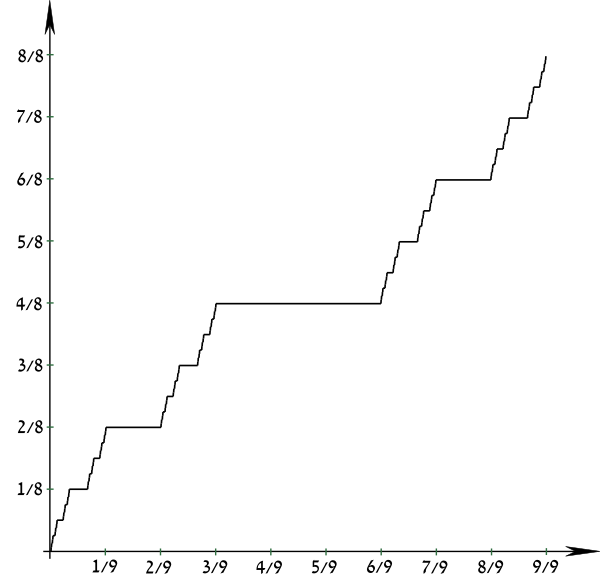
\includegraphics[scale=0.3]{img/devils_staircase.png}
      \caption{Plot} 
      \label{fig:devils_staircase}
    \end{figure}
  \end{definition} 

  \begin{theorem}
    $\phi$ is a nondecreasing, continuous function s.t. $\phi^\prime (x) = 0$ for all $x \in O$ and $m(O) = 1$. 
  \end{theorem}
  \begin{proof}
    Listed. 
    \begin{enumerate}
      \item \textit{Increasing}. $\phi$ is increasing on each $O_k$, and so on $O$. Then, it is also increasing on $C$ by definition. 
      \item \textit{Continuity}. If $x \in C$, it lies between 2 intervals of $O_k$ for any $k$. The difference in function values between 2 neighboring intervals of $O_k$ is $2^{-k}$, so $\phi$ is continuous. 
      \item \textit{Derivative}. The derivative is $0$ because it is constant around an interval. 
    \end{enumerate}
  \end{proof}

  \begin{theorem}[]
    Define $\psi (x) = \phi(x) + x$. Then, 
    \begin{enumerate}
      \item $\psi$ is continuous and strictly increasing. 
      \item $\psi$ maps $C$ into a set of positive measure. 
      \item $\psi$ maps some subset of $C$ into a nonmeasurable set. 
    \end{enumerate}
  \end{theorem}
  \begin{proof}
    Listed. 
    \begin{enumerate}
      \item Continuity is from sum of continuous functions, and strictly increasing since $\phi$ is nondecreasing and $x$ is strictly increasing. 
      \item We know that $\psi([0, 1]) = [0, 2]$ and $m(\psi(O))= 1$, where for each interval $I_j \subset O$, $m(\psi(I_j)) = \ell(I_j)$. Therefore, $m(\psi(C)) = 1$. 
      \item Since $\psi$ is strictly increasing, there exists a continuous inverse $\psi^{-1}$. Find $Z \subset \psi(C)$ that is nonmeasurable, which we can do from the previous theorem. Then, there exists $E \subset C$ s.t. $\psi(E) = Z$, and $E$ is not Borel since if it were, then $Z$ would be Borel, too. 
    \end{enumerate}
  \end{proof}

